\section{Principio di funzionamento}
\subsection{L'apparato circolatorio}
L'apparato circolatorio è fondamentale per la sopravvivenza di tutte le cellule del corpo umano. Il suo compito è quello di provvedere ai bisogni dei tessuti, mantenendo un ambiente adeguato alla sopravvivenza delle cellule che li compongono (omeostasi)\cite{Cevese2002}. 
L'apparato cardiocircolatorio è composto da tre elementi fondamentali:
\begin{enumerate}
\item il sangue, una sospensione di cellule e frazioni cellulari (globuli rossi, globuli bianchi e piastrine) in un liquido acquoso (plasma), contenente proteine e elettroliti;
\item il cuore, un muscolo che, agendo come una pompa, fornisce al sangue la pressione necessaria per poter circolare in tutto il corpo;
\item i vasi sanguigni, un circuito di condotti che permettono al sangue di scorrere lungo tutto il corpo.
\end{enumerate}
Grazie a questo apparato, è possibile trasportare gas respiratori (anidride carbonica e ossigeno), sostanze nutritive (glucosio, aminoacidi, acidi grassi) e messaggi chimici (ormoni) verso tutte le cellule dei tessuti. Inoltre, vengono raccolte e eliminate tutte le sostanze di scarto, prodotte  dalle reazioni chimiche che avvengono nelle cellule. La loro eliminazione è affidata a organi specializzati, come i reni e il fegato, che agiscono come dei filtri, oppure ai polmoni, che permettono lo scambio gassoso, eliminando l'anidride carbonica e assimilando l'ossigeno. Il sangue è anche un elemento che permette la termoregolazione all'interno degli esseri viventi: variando il flusso nei tessuti più esterni è possibile controllare la dispersione del calore corporeo con l'ambiente esterno. Il volume e il flusso di sangue nei tessuti viene controllato dall'azione coordinata di cuore e vasi sanguigni, che insieme permettono di regolarne l'apporto.

All'interno del sistema circolatorio è possibile identificare diverse tipologie di vasi che si differenziano per struttura e funzione. Si suddividono in: arterie, arteriole, capillari, venule e vene. Ciononostante, tutte le pareti vasali sono costituite, in proporzioni variabili, da: endotelio, fibre collagene, fibre elastiche e fibre muscolari lisce. 
Le \textit{arterie} hanno il compito di trasportare il sangue ad alta pressione dal cuore verso i tessuti. A tal fine, analizzando la loro struttura, si possono notare delle pareti vascolari molto resistenti e flessibili. L'arteria principale è l'aorta, che si estende dal ventricolo sinistro  fino alla biforcazione iliaca e permette al sangue arterioso (ricco di ossigeno) di raggiungere i vasi arteriosi di calibro inferiore.
Il sistema arterioso termina con le \textit{arteriole}, che regolano la quantità di sangue immessa nei capillari. Per questo motivo, presentano forti pareti muscolari, che ne permettono la dilatazione o la costrizione.
I \textit{capillari} presentano invece pareti molto sottili e porose, che li rendono permeabili all'acqua e ad alcune molecole. Infatti, a loro è affidato il compito di permettere lo scambio di fluidi e sostanze tra il sangue e il liquido interstiziale delle cellule. 
Infine, le \textit{venule} raccolgono il sangue dei capillari e gradualmente si fondono nelle vene, condotti più larghi, adibiti al trasporto del sangue verso il cuore. In aggiunta, esse costituiscono un'importante riserva ematica, contenendone circa il 65\%. Le vene si differenziano dalle arterie per avere pareti più sottili, in quanto adibite al trasporto di sangue con una minore pressione \cite{Armentano2019}. In aggiunta, alcune vene presenti soprattutto nelle gambe, presentano delle valvole a \textit{nido di rondine}, che impediscono reflusso del sangue. 

Analizzando la complessa rete vascolare, è possibile identificare due sotto-circuiti principali \Fig~\ref{fig:SistemaCircolatorio}:
\begin{figure}[h]
	\centering
	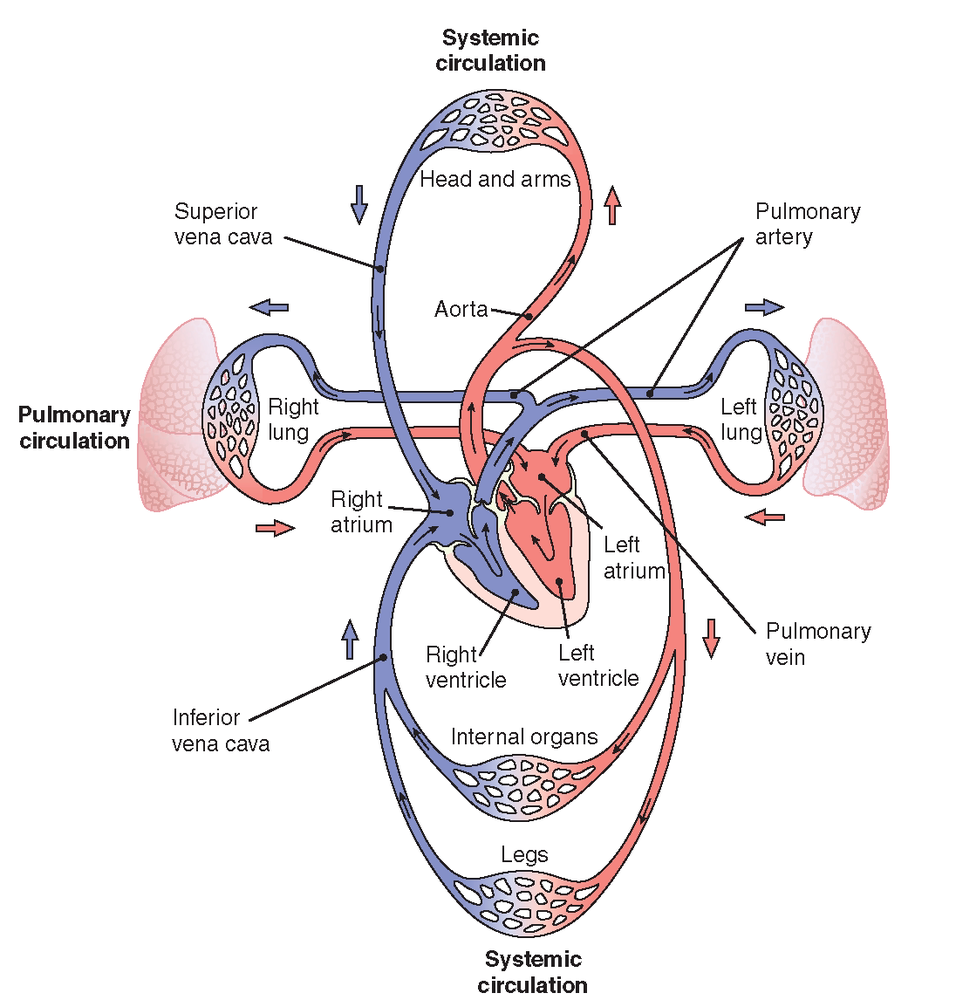
\includegraphics[width=0.7\linewidth]{ImageFiles/Fotopletismografia/SistemaCircolatorio}
	\caption{Rappresentazione del sistema circolatorio.}
	\label{fig:SistemaCircolatorio}
\end{figure}
\begin{itemize}
	\item la \textit{circolazione polmonare}, o piccola circolazione, che include i vasi che dal ventricolo destro del cuore si capillarizza a livello degli alveoli polmonari e ritorna al cuore nell'atrio sinistro tramite le \textit{vene polmonari};
	\item la \textit{circolazione sistemica}, o grande circolazione, che permette al sangue di scorrere dal ventricolo sinistro all'interno dell'\textit{aorta} per poi raggiungere tutto il corpo e ritornare, grazie alla \textit{vena cava}, all'atrio destro.
\end{itemize}
Tuttavia, la distinzione nei due circuiti è puramente concettuale \todo{non mi piace molto} e, in realtà, i due sono strettamente interdipendenti \cite{Cutfield1983}. In effetti, il sangue deossigenato, proveniente \todo{cfr. fonte: https://www.kenhub.com/en/library/anatomy/circulatory-system} dalla circolazione sistemica, ritorna all'atrio destro attraverso la vena cava superiore e inferiore. Durante la fase di \textit{diastole}, scorre nel ventricolo destro attraverso la \textit{valvola tricuspide} e successivamente, grazie alla contrazione del ventricolo (fase di \textit{diastole}), viene spinto nell'arteria polmonare destra e sinistra, che portano il sangue ai polmoni. Grazie ai capillari polmonari avviene il processo di \textit{ematosi}, durante il quale il sangue assimila ossigeno e cede anidride carbonica. Le vene polmonari raccolgono il sangue appena ossigenato e lo conducono nell'atrio sinistro. A questo punto, si ha il punto di passaggio dalla circolazione polmonare alla circolazione sistemica. Dall'atrio destro, attraverso la \textit{valvola bicuspide}, il sangue procede verso il ventricolo sinistro nella la fase di diastole. In seguito, la sistole costringe il sangue nell'aorta che diramandosi fino ai capillari permette la perfusione in tutti i tessuti. Infine, il sangue viene riportato all'atrio destro attraverso le vene cave superiore e inferiore. Il ciclo può ora ripartire. 

\subsection{La circolazione: Pressione, Flusso e Resistenza}
\todo{sistemare immagine e iniziare discorso su pressione}
 \Fig~\ref{fig:PressioneSangue} 
 \begin{figure}[h]
 	\centering
 	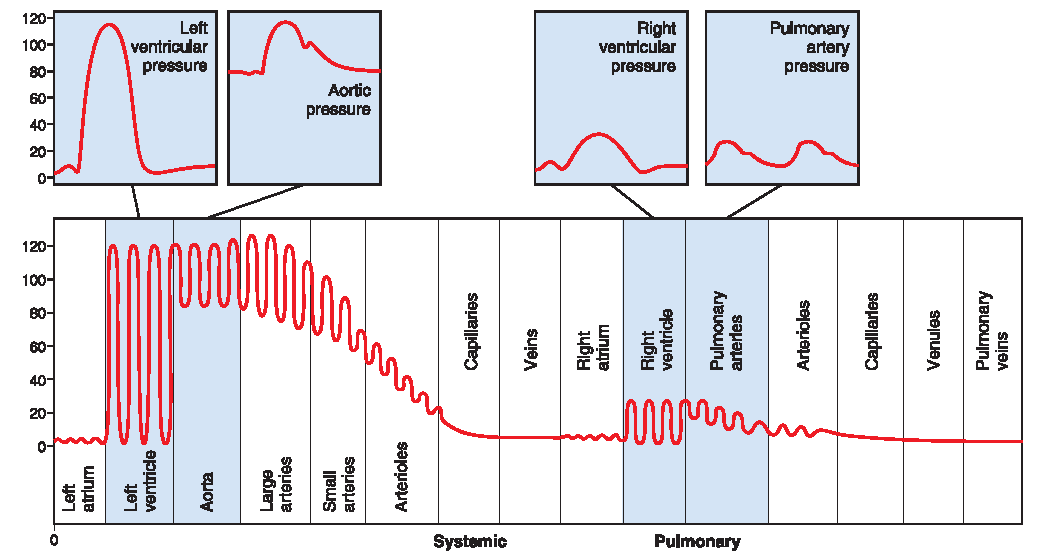
\includegraphics[width=0.7\linewidth]{ImageFiles/Fotopletismografia/PressioneSangue}
 	\caption{todo}
 	\label{fig:PressioneSangue}
 \end{figure}
\pagebreak